\documentclass{beamer}

\mode<presentation>						% Set options
{
  \usetheme{Hannover}					% Set theme
  \usecolortheme{rose} 				% Set colors
  \usefonttheme{structurebold}  				% Set font theme
  \setbeamertemplate{caption}[numbered]	% Set caption to be numbered
}

% Uncomment this to have the outline at the beginning of each section highlighted.
\AtBeginSection[]
{
  \begin{frame}
    \tableofcontents[currentsection]
  \end{frame}
}

\usepackage[varg]{txfonts}
\usepackage[T1]{fontenc}
\usepackage[sfdefault,scaled=0.95]{FiraSans}
\usepackage[small,euler-digits]{eulervm}
\usepackage{inconsolata}
\usepackage{textcomp}
\usepackage{graphicx}					% For including figures
\usepackage{booktabs}					% For table rules
\usepackage{hyperref}					% For cross-referencing

\title[Towards Categorical Metadata]{Towards Categorical Metadata\\ for Unreduced Climate Observations}
\author[C.~Grainger]{Colton Grainger}
\institute{University of Colorado}
\date{\today}

\begin{document}

\begin{frame}
    \titlepage
    \vfill
    \begin{figure}
        \includegraphics[height=5em]{img/}
        
\includegraphics[height=4.5em]{img/CISL-contemp-logo-blue-square}\hspace{0.5em}
        
\includegraphics[height=5em]{img/cu-logo}\hspace{0.5em}
        
\includegraphics[height=5em]{img/nsf-logo}
    \end{figure}
\end{frame}

\section{Status Quo}
\section{Plan Text}

\begin{frame}
    \begin{itemize}
        \item Gather images at a \textbf{single resource}.
        \item Establish a \textbf{common description framework} for image metadata.
        \item Provide \textbf{bulk, programmatic access} to image subsets.
    \end{itemize}
\end{frame}

\section{Basic Methods}

\begin{frame}
	\begin{columns}
		\column{.33\textwidth}
        MySQL schema. Makefile.

        \column{.33\textwidth}
        Agnostic ingest scripts.
        \texttt{assign\_uuid()}.
        Bundle metadata.

        \column{.33\textwidth}
        \texttt{rda.ucar.edu/i/<uuid>}
	\end{columns}
\end{frame}

\section{Future Work}

\begin{frame}
	\begin{columns}
		\column{.33\textwidth}
        RELAX NG validator.

        \column{.33\textwidth}
        Python pandas interface.
        Query methods.

        \column{.33\textwidth}
        \texttt{rda.ucar.edu/i/<query>}
	\end{columns}
\end{frame}

\section{References}
\begin{frame}
    \begin{figure}
        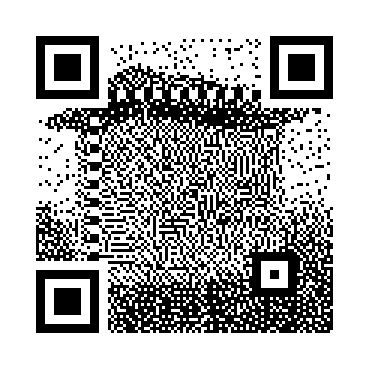
\includegraphics[width=0.4\textwidth]{img/meteo_qrcode}
        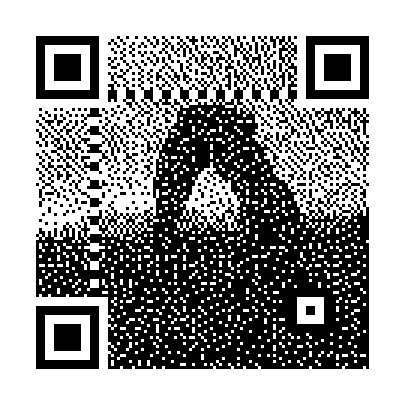
\includegraphics[width=0.4\textwidth]{img/arch_qrcode}
        
\includegraphics[width=0.4\textwidth]{img/brohan_qrcode}
    \end{figure}
\end{frame}

\end{document}
